\documentclass{beamer}

\usepackage{algorithm} %
\usepackage{algpseudocode} %
\usepackage{tikz} %grahps 
\usetikzlibrary{automata, arrows, positioning, decorations.pathreplacing}


\title{Résolution de jeux de sûreté joués sur graphes}
\author{Huylenbroeck Florent}
\institute{UMONS}
\date{25 novembre 2022}
\begin{document}

\frame{\titlepage}

\begin{frame}
\frametitle{Sommaire}
\tableofcontents
\end{frame}

\section{Jeux joués sur graphes}
\begin{frame}
\frametitle{Jeux joués sur graphes}
Objectif : modéliser les interactions d'un système et de son environnement.\\[3mm]

\noindent
\begin{minipage}[t]{.45\textwidth}
\textbf{Sûreté} : éviter certaines configurations.\\
\emph{Eviter un deadlock, qu'une valeur soit nulle, ...}
\end{minipage}
\hfill\vline\hfill
\begin{minipage}[t]{.45\textwidth}
\textbf{Atteignabilité} : atteindre certaines configurations.\\
\emph{Au moins une requête reçoit une réponse, une variable est initialisée ...}
\end{minipage}\\[2mm]
\end{frame}


\begin{frame}
\frametitle{Jeux joués sur graphes}
Une jeu joué sur graphe est défini par les ensembles $V_s$, $V_e$, $E$ formant une \emph{arène}, ainsi que $F$ et $I$.
\begin{figure}[h]
\centering
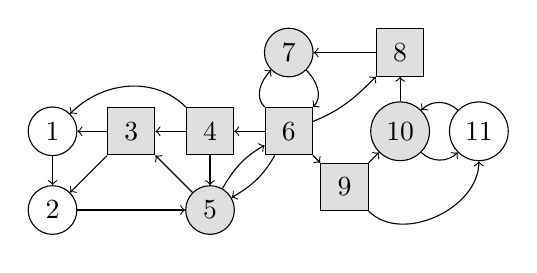
\begin{tikzpicture}[	
						node distance={10mm},
						round/.style = {draw, circle, minimum size=5mm},
						ground/.style = {draw, fill=gray!25, circle, minimum size=5mm},						
						square/.style = {draw, rectangle, minimum size=6mm},
						gsquare/.style = {draw, fill=gray!25, rectangle, minimum size=6mm}
					]
\node[round] (1) {$1$};
\node[round] (2) [below of=1] {$2$};
\node[gsquare] (3) [right of=1] {$3$};
\node[gsquare] (4) [right of=3] {$4$};
\node[ground] (5) [below of=4] {$5$};
\node[gsquare] (6) [right of=4] {$6$};
\node[ground] (7) [above of=6] {$7$};
\node[gsquare] (9) [below right of=6] {$9$};
\node[ground] (10) [above right of=9] {$10$};
\node[gsquare] (8) [above of=10] {$8$};
\node[round] (11) [right of=10] {$11$};

\draw[->] (1) -- (2);
\draw[->] (2) -- (5);
\draw[->] (3) -- (1);
\draw[->] (3) -- (2);
\draw[->] (4) to [out=135, in=45] (1);
\draw[->] (4) -- (3);
\draw[->] (4) -- (5);
\draw[->] (5) -- (3);
\draw[->] (5) to [out=60, in=210] (6);
\draw[->] (6) -- (4);
\draw[->] (6) to [out=240, in=30] (5);
\draw[->] (6) to [out=135, in=225] (7);
\draw[->] (6) -- (9);
\draw[->] (6) to [out=22, in=225] (8);
\draw[->] (7) to [out=315, in=45] (6);
\draw[->] (8) -- (7);
\draw[->] (9) -- (10);
\draw[->] (9) to [out=315, in=270] (11);
\draw[->] (10) -- (8);
\draw[->] (10) to [out=315, in=225] (11);
\draw[->] (11) to [out=135, in=45] (10);
\end{tikzpicture}
%\caption{Exemple d'une arène}
\label{fig:arena}
\end{figure}

\begin{minipage}{.15\textwidth}
\begin{figure}[h]
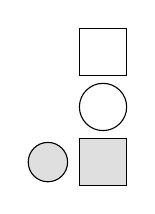
\begin{tikzpicture}
[	
						node distance={7mm},
						round/.style = {draw, circle, minimum size=6mm},
						ground/.style = {draw, fill=gray!25, circle, minimum size=5mm},						
						square/.style = {draw, rectangle, minimum size=6mm},
						gsquare/.style = {draw, fill=gray!25, rectangle, minimum size=6mm}
					]
\node[square] (1) {};
\node[round] (2) [below of=1] {};
\node[gsquare] (3) [below of=2] {};
\node[ground] (4) [left of=3] {};
\end{tikzpicture}
\end{figure}
\end{minipage}
\begin{minipage}{.60\textwidth}
Sommets du système ($V_s$).\\[2mm]
Sommets de l'environnement ($V_e$).\\[2mm]
Sommets correspondant à l'objectif ($F$).
\end{minipage}\\[3mm]
Les arcs reliant ces sommets représentent l'ensemble $E$.
\end{frame}


\begin{frame}
\frametitle{Jeux joués sur graphes}
Au début de la partie, un \emph{pion} est placé sur un sommet de $I$ dans l'arène.\\
Le joueur possédant le sommet sur lequel est le pion décide du prochain coup.\\[10mm]
$\rightarrow$ Il faut trouver une stratégie gagnante selon l'objectif.
\end{frame}

\section{Cas fini}
\begin{frame}
\frametitle{Cas fini} %exemple %terminer par => attracteur
Les ensembles $V_s$ et $V_e$ sont finis.\\[3mm]
On va déterminer les sommets à partir desquels le système peut toujours remplir son objectif. Si tous ces sommets sont dans $I$, alors le système pourra toujours respecter la spécification.\\[3mm]
Trouver cet ensemble de sommet, appelé \emph{ensemble gagnant}, est possible, par exemple en construisant un \emph{attracteur}.
\end{frame}

\subsection{Attracteurs}
\begin{frame}
\frametitle{Attracteur : définition}
\begin{block}{$i^e$-attracteur}
Soit un sous-ensemble de sommets $F$ d'une arène. Le \emph{$i^e$-attracteur} pour un joueur vers $F$ est l'ensemble des sommets tel que, depuis tous les sommets de cet attracteur, le joueur peut forcer une visite d'un sommet de $F$ en au plus $i$ coups.
\end{block}

\begin{block}{attracteur}
Soit un sous-ensemble de sommets $F$ d'une arène. L'\emph{attracteur} vers ces sommets pour un joueur est l'ensemble de sommets tels que le joueur peut forcer une visite d'un sommet de $F$ depuis n'importe lequel de ces sommets.
\end{block}
\end{frame}

\begin{frame}
\frametitle{Attracteur : calcul}
L'idée est de calculer la série des $i^e$-attracteurs vers $F$ jusqu'à ce qu'augmenter $i$ n'ajoute plus de sommets à l'attracteur.

\begin{equation}
\label{eq:induction}
\begin{split}
Attr^0_{s}(F)&=F\\
Attr^{i+1}_{s}(F)&=Attr^i_{s}(F)\\
			&\cup \{v'\in V_s\text{ }|\text{ }\exists(v,v')\in E:v\in Attr^i_{s}(F)\}\\
			&\cup \{v'\in V_e\text{ }|\text{ }\forall(v,v')\in E:v\in Attr^i_{s}(F)\}
\end{split}
\end{equation}\\
On obtiendra ainsi $Attr_{s}^0(F)\subseteq Attr_{s}^1(F) \subseteq ...=Attr_s(F)$\\[3mm]
La complexité de cette construction est en \alert{$O(m+n)$} pour une arène composée de $n$ sommets et $m$ arcs.
\end{frame}

\subsection{Stratégie gagnante}
\begin{frame}
\frametitle{Dualité jeux d'atteignabilité et sûreté}
\textbf{Jeux d'atteignabilité}\\
Construire l'attracteur vers l'ensemble objectif $F$ pour le système donne immédiatement une stratégie gagnante pour celui-ci : à chaque coup, déplacer le pion d'un sommet de $Attr_{s}^{i+1}(F)$ vers un sommet dans $Attr_{s}^{i}(F)$\\[3mm]

$\rightarrow$ La construction opposée nous donne une stratégie gagnante pour un jeu de sûreté.\\[3mm]

\textbf{Jeux de sûreté}\\
Construire l'attracteur pour l'environnement vers les sommets hors de l'objectif $F$ indique au système quels sommets éviter. Il obtient ainsi une stratégie gagnante en restant hors de cet attracteur à chaque coup.
\end{frame}

\subsection{Exemple}
\begin{frame}
\frametitle{Exemple}
Calculons l'attracteur de l'environnement vers les sommets hors de l'objectif pour l'arène précédente. Les sommets du $0^e$-attracteur sont entourés en rouge.
\begin{figure}[h]
\centering
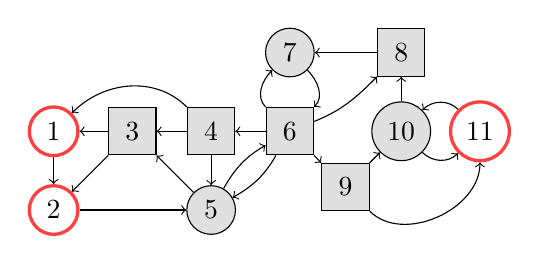
\begin{tikzpicture}[	
						node distance={10mm},
						round/.style = {draw, circle, minimum size=5mm},
						ground/.style = {draw, fill=gray!25, circle, minimum size=5mm},						
						square/.style = {draw, rectangle, minimum size=6mm},
						gsquare/.style = {draw, fill=gray!25, rectangle, minimum size=6mm}
					]
\node[round] (1) [draw=red!75, very thick]{$1$};
\node[round] (2) [below of=1, draw=red!75, very thick] {$2$};
\node[gsquare] (3) [right of=1] {$3$};
\node[gsquare] (4) [right of=3] {$4$};
\node[ground] (5) [below of=4] {$5$};
\node[gsquare] (6) [right of=4] {$6$};
\node[ground] (7) [above of=6] {$7$};
\node[gsquare] (9) [below right of=6] {$9$};
\node[ground] (10) [above right of=9] {$10$};
\node[gsquare] (8) [above of=10] {$8$};
\node[round] (11) [right of=10, draw=red!75, very thick] {$11$};

\draw[->] (1) -- (2);
\draw[->] (2) -- (5);
\draw[->] (3) -- (1);
\draw[->] (3) -- (2);
\draw[->] (4) to [out=135, in=45] (1);
\draw[->] (4) -- (3);
\draw[->] (4) -- (5);
\draw[->] (5) -- (3);
\draw[->] (5) to [out=60, in=210] (6);
\draw[->] (6) -- (4);
\draw[->] (6) to [out=240, in=30] (5);
\draw[->] (6) to [out=135, in=225] (7);
\draw[->] (6) -- (9);
\draw[->] (6) to [out=22, in=225] (8);
\draw[->] (7) to [out=315, in=45] (6);
\draw[->] (8) -- (7);
\draw[->] (9) -- (10);
\draw[->] (9) to [out=315, in=270] (11);
\draw[->] (10) -- (8);
\draw[->] (10) to [out=315, in=225] (11);
\draw[->] (11) to [out=135, in=45] (10);
\end{tikzpicture}
%\caption{Exemple d'une arène}
\end{figure}
\end{frame}

\begin{frame}
\frametitle{Exemple}
$1^{er}$-attracteur
\begin{figure}[h]
\centering
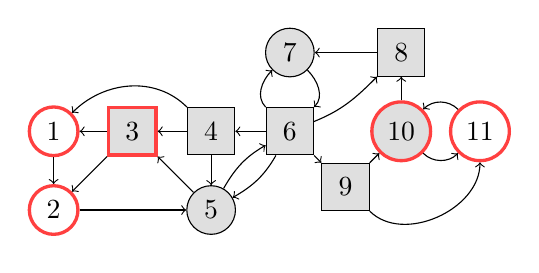
\begin{tikzpicture}[	
						node distance={10mm},
						round/.style = {draw, circle, minimum size=5mm},
						ground/.style = {draw, fill=gray!25, circle, minimum size=5mm},						
						square/.style = {draw, rectangle, minimum size=6mm},
						gsquare/.style = {draw, fill=gray!25, rectangle, minimum size=6mm}
					]
\node[round] (1) [draw=red!75, very thick]{$1$};
\node[round] (2) [below of=1, draw=red!75, very thick] {$2$};
\node[gsquare] (3) [right of=1, draw=red!75, very thick] {$3$};
\node[gsquare] (4) [right of=3] {$4$};
\node[ground] (5) [below of=4] {$5$};
\node[gsquare] (6) [right of=4] {$6$};
\node[ground] (7) [above of=6] {$7$};
\node[gsquare] (9) [below right of=6] {$9$};
\node[ground] (10) [above right of=9, draw=red!75, very thick] {$10$};
\node[gsquare] (8) [above of=10] {$8$};
\node[round] (11) [right of=10, draw=red!75, very thick] {$11$};

\draw[->] (1) -- (2);
\draw[->] (2) -- (5);
\draw[->] (3) -- (1);
\draw[->] (3) -- (2);
\draw[->] (4) to [out=135, in=45] (1);
\draw[->] (4) -- (3);
\draw[->] (4) -- (5);
\draw[->] (5) -- (3);
\draw[->] (5) to [out=60, in=210] (6);
\draw[->] (6) -- (4);
\draw[->] (6) to [out=240, in=30] (5);
\draw[->] (6) to [out=135, in=225] (7);
\draw[->] (6) -- (9);
\draw[->] (6) to [out=22, in=225] (8);
\draw[->] (7) to [out=315, in=45] (6);
\draw[->] (8) -- (7);
\draw[->] (9) -- (10);
\draw[->] (9) to [out=315, in=270] (11);
\draw[->] (10) -- (8);
\draw[->] (10) to [out=315, in=225] (11);
\draw[->] (11) to [out=135, in=45] (10);
\end{tikzpicture}
%\caption{Exemple d'une arène}
\end{figure}
$2^{e}$-attracteur
\begin{figure}[h]
\centering
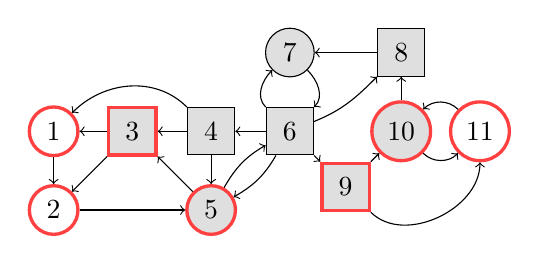
\begin{tikzpicture}[	
						node distance={10mm},
						round/.style = {draw, circle, minimum size=5mm},
						ground/.style = {draw, fill=gray!25, circle, minimum size=5mm},						
						square/.style = {draw, rectangle, minimum size=6mm},
						gsquare/.style = {draw, fill=gray!25, rectangle, minimum size=6mm}
					]
\node[round] (1) [draw=red!75, very thick]{$1$};
\node[round] (2) [below of=1, draw=red!75, very thick] {$2$};
\node[gsquare] (3) [right of=1, draw=red!75, very thick] {$3$};
\node[gsquare] (4) [right of=3] {$4$};
\node[ground] (5) [below of=4, draw=red!75, very thick] {$5$};
\node[gsquare] (6) [right of=4] {$6$};
\node[ground] (7) [above of=6] {$7$};
\node[gsquare] (9) [below right of=6, draw=red!75, very thick] {$9$};
\node[ground] (10) [above right of=9, draw=red!75, very thick] {$10$};
\node[gsquare] (8) [above of=10] {$8$};
\node[round] (11) [right of=10, draw=red!75, very thick] {$11$};

\draw[->] (1) -- (2);
\draw[->] (2) -- (5);
\draw[->] (3) -- (1);
\draw[->] (3) -- (2);
\draw[->] (4) to [out=135, in=45] (1);
\draw[->] (4) -- (3);
\draw[->] (4) -- (5);
\draw[->] (5) -- (3);
\draw[->] (5) to [out=60, in=210] (6);
\draw[->] (6) -- (4);
\draw[->] (6) to [out=240, in=30] (5);
\draw[->] (6) to [out=135, in=225] (7);
\draw[->] (6) -- (9);
\draw[->] (6) to [out=22, in=225] (8);
\draw[->] (7) to [out=315, in=45] (6);
\draw[->] (8) -- (7);
\draw[->] (9) -- (10);
\draw[->] (9) to [out=315, in=270] (11);
\draw[->] (10) -- (8);
\draw[->] (10) to [out=315, in=225] (11);
\draw[->] (11) to [out=135, in=45] (10);
\end{tikzpicture}
%\caption{Exemple d'une arène}
\end{figure}
\end{frame}

\begin{frame}
\frametitle{Exemple}
$3^{e}$-attracteur, $4^e$-attracteur, ...
\begin{figure}[h]
\centering
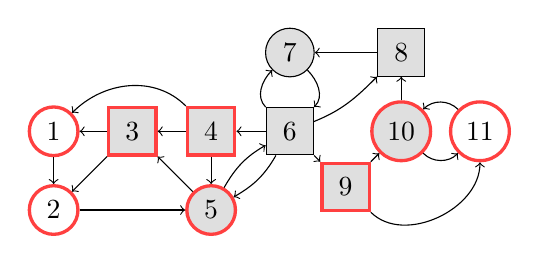
\begin{tikzpicture}[	
						node distance={10mm},
						round/.style = {draw, circle, minimum size=5mm},
						ground/.style = {draw, fill=gray!25, circle, minimum size=5mm},						
						square/.style = {draw, rectangle, minimum size=6mm},
						gsquare/.style = {draw, fill=gray!25, rectangle, minimum size=6mm}
					]
\node[round] (1) [draw=red!75, very thick]{$1$};
\node[round] (2) [below of=1, draw=red!75, very thick] {$2$};
\node[gsquare] (3) [right of=1, draw=red!75, very thick] {$3$};
\node[gsquare] (4) [right of=3, draw=red!75, very thick] {$4$};
\node[ground] (5) [below of=4, draw=red!75, very thick] {$5$};
\node[gsquare] (6) [right of=4] {$6$};
\node[ground] (7) [above of=6] {$7$};
\node[gsquare] (9) [below right of=6, draw=red!75, very thick] {$9$};
\node[ground] (10) [above right of=9, draw=red!75, very thick] {$10$};
\node[gsquare] (8) [above of=10] {$8$};
\node[round] (11) [right of=10, draw=red!75, very thick] {$11$};

\draw[->] (1) -- (2);
\draw[->] (2) -- (5);
\draw[->] (3) -- (1);
\draw[->] (3) -- (2);
\draw[->] (4) to [out=135, in=45] (1);
\draw[->] (4) -- (3);
\draw[->] (4) -- (5);
\draw[->] (5) -- (3);
\draw[->] (5) to [out=60, in=210] (6);
\draw[->] (6) -- (4);
\draw[->] (6) to [out=240, in=30] (5);
\draw[->] (6) to [out=135, in=225] (7);
\draw[->] (6) -- (9);
\draw[->] (6) to [out=22, in=225] (8);
\draw[->] (7) to [out=315, in=45] (6);
\draw[->] (8) -- (7);
\draw[->] (9) -- (10);
\draw[->] (9) to [out=315, in=270] (11);
\draw[->] (10) -- (8);
\draw[->] (10) to [out=315, in=225] (11);
\draw[->] (11) to [out=135, in=45] (10);
\end{tikzpicture}
%\caption{Exemple d'une arène}
\end{figure}
Au terme de la quatrième itération, aucun sommet n'est ajouté à l'attracteur.\\[3mm]
$\rightarrow$ La stratégie gagnante pour le système est de jouer ses coups vers les sommets $6$, $7$ et $8$. Si le pion est initialement placé sur un de ces sommets, le système gagne.
\end{frame}

\section{Cas infini}
\begin{frame}
\frametitle{Cas infini} %exemple %meilleur def de W %3 étapes
On autorise $V_s$ et $V_e$ à être infinis.\\[3mm]

Un algorithme linéaire en terme d'arcs et de sommets aurait une complexité \alert{infinie}.\\[3mm]
$\rightarrow$ Il faut passer par une étape d'abstraction.
\end{frame}

\subsection{Représentation régulière du problème}
\begin{frame}
\frametitle{Alphabet, mots et langage}
\begin{block}{Alphabet, mot et langage}
Un alphabet $\Sigma$ est un ensemble de caractères. Un mot sur cet alphabet est une suite de caractères de cet alphabet. Le mot vide est noté $\epsilon$. L'ensemble des mots sur un alphabet est noté $\Sigma^*$.\\
Un langage $L$ sur $\Sigma$ est un sous-ensemble de $\Sigma^*$\\[3mm]
\end{block}
\begin{exampleblock}{Exemple}
Le langage $L=\{u\in\Sigma^*$ $|$ $u=ab^n, n\in\mathbb{N}_0\}$ est le langage sur $\Sigma=\{a,b\}$ des mots commencant par $a$, suivi d'une répétition de $b$.
\end{exampleblock}
\end{frame}

\begin{frame}
\frametitle{Automates}
\begin{block}{Automate fini}
\noindent Un \emph{automate} fini est un 5-uple $\mathcal{A}=(Q,\Sigma,\delta,q_0,F)$ où 
\begin{itemize}
	\item $Q$ est un ensemble fini, non vide, d'états.
	\item $\Sigma$ est l'alphabet lu par l'automate.
	\item $\delta$ est une fonction $Q\times\Sigma\to Q$ appelée \emph{fonction de transition} de l'automate. L'expression $\delta(q_1,u)=q_2$ indique que l'automate transitionne de l'état $q_1$ à l'état $q_2$ quand le mot $u\in\Sigma^*$ est lu depuis l'état $q_1$.
	\item $q_0\subseteq Q$ est l'ensemble des états initiaux.
	\item $F\subseteq Q$ est l'ensemble des états finaux.
\end{itemize}
\end{block}
\begin{exampleblock}{Exemple}
\begin{figure}[H]
\centering
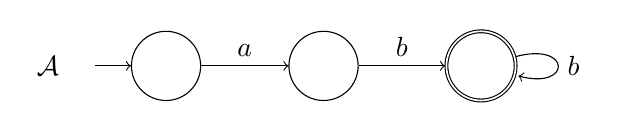
\begin{tikzpicture} [
						node distance=2cm, 
						auto,
						every initial by arrow/.style={->}
					]
					
\node (1) [state, initial, initial text=] {};
\node (2) [state, right of=1] {};
\node (3) [state, accepting, right of=2] {};
\node (0) [left of=1, node distance=1.5cm] {$\mathcal{A}$};

\path[->]
	(1) edge node {$a$}   (2)
	(2) edge node {$b$}   (3)
	(3) edge [loop right] node {$b$} ();
\end{tikzpicture}\\
$\mathcal{A}$ est l'automate qui accepte le langage de l'exemple précédent.
\end{figure}
\end{exampleblock}
\end{frame}

\begin{frame}
\frametitle{Transducteurs}
\begin{block}{Transducteur}
Un transducteur est un automate fini dont les transitions se font par des paires de caractères, dont les composantes appartiennent chacune à un alphabet respectif. Il permet de définir une relation entre deux langages.
\end{block}
\begin{exampleblock}{Exemple}
\begin{figure}[H]
\centering
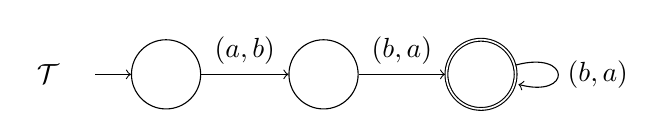
\begin{tikzpicture} [
						node distance=2cm, 
						auto,
						every initial by arrow/.style={->}
					]
					
\node (1) [state, initial, initial text=] {};
\node (2) [state, right of=1] {};
\node (3) [state, accepting, right of=2] {};
\node (0) [left of=1, node distance=1.5cm] {$\mathcal{T}$};

\path[->]
	(1) edge node {$(a,b)$}   (2)
	(2) edge node {$(b,a)$}   (3)
	(3) edge [loop right] node {$(b,a)$} ();
\end{tikzpicture}
\end{figure}
$\mathcal{T}$ est le transducteur qui permet d'établir la relation "d'inversion" du langage de $\mathcal{A}$ de l'exemple précédent.
\end{exampleblock}
\end{frame}


\begin{frame}
\frametitle{Exemple de jeu de sûreté infini}
Introduisons maintenant un exemple de jeu de sûreté joué sur une arène infinie
\begin{figure}[H]
\centering
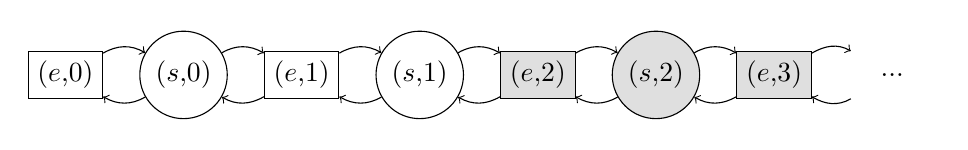
\begin{tikzpicture}[
						node distance={15mm},
						round/.style = {draw, circle, minimum size=6mm},
						cround/.style = {draw, fill=gray!25, circle, minimum size=6mm},
						noround/.style = {circle, minimum size=12mm},
						square/.style = {draw, rectangle, minimum size=6mm},
						csquare/.style = {draw, fill=gray!25, rectangle, minimum size=6mm},
					]
					
\node[square] (1) {($e$,$0$)};
\node[round] (2) [right of=1] {($s$,$0$)};
\node[square] (3) [right of=2] {($e$,$1$)};
\node[round] (4) [right of=3] {($s$,$1$)};
\node[csquare] (5) [right of=4] {($e$,$2$)};
\node[cround] (6) [right of=5] {($s$,$2$)};
\node[csquare] (7) [right of=6] {($e$,$3$)};
\node[noround] (8) [right of=7] {...};

\draw[->] (1) to [out=30,in=150] (2);
\draw[->] (2) to [out=210,in=330] (1);
\draw[->] (2) to [out=30,in=150] (3);
\draw[->] (3) to [out=210,in=330] (2);
\draw[->] (3) to [out=30,in=150] (4);
\draw[->] (4) to [out=210,in=330] (3);
\draw[->] (4) to [out=30,in=150] (5);
\draw[->] (5) to [out=210,in=330] (4);
\draw[->] (5) to [out=30,in=150] (6);
\draw[->] (6) to [out=210,in=330] (5);
\draw[->] (6) to [out=30,in=150] (7);
\draw[->] (7) to [out=210,in=330] (6);
\draw[->] (7) to [out=30,in=150] (8);
\draw[->] (8) to [out=210,in=330] (7);

\end{tikzpicture}
\end{figure}
Arène infinie, fermée à gauche. Le système ne peut déplacer le pion que vers la droite ou ne pas le déplacer. L'environnement ne peut le déplacer que vers la gauche ou pas du tout.\\[3mm]
L'ensemble objectif $F$ correspond aux sommets dont le numéro est supérieur à $2$.\\[3mm]
Initialement, le pion est placé sur un sommet du système dans $F$.
\end{frame}

\begin{frame}
\frametitle{Représentation régulière}
Afin de représenter notre jeu de sûreté sous forme d'automates, il faut trouver un encodage, afin de définir l'alphabet utilisé par les automates.\\[3mm]
Pour cet exemple, l'alphabet choisit est $\Sigma=\{s,e,i\}$. Les sommets seront encodés par les mots $u\in\{si^n,ei^n, n\in\mathbb{N}\}$

\begin{exampleblock}{Exemple}
Le premier sommet de l'ensemble $F$ sera encodé par $eii$, le sommet à sa droite $sii$, etc.
\end{exampleblock}
\end{frame}

\begin{frame}
\frametitle{Représentation régulière}
L'automate $\mathcal{A}_{V_s}$ représente les sommets du système.
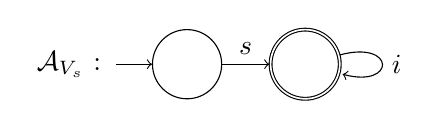
\begin{tikzpicture} [
						node distance=1.5cm, 
						auto,
						every initial by arrow/.style={->}
					]
					
\node (1) [state, initial, initial text=] {};
\node (2) [state, accepting, right of=1] {};
\node (0) [left of=1] {$\mathcal{A}_{V_s}$ :};

\path[->]
	(1) edge node {$s$}   (2)
	(2) edge [loop right] node {$i$} ();
\end{tikzpicture}\\[3mm]
Le transducteur $\mathcal{T}_E$ représente les transitions.
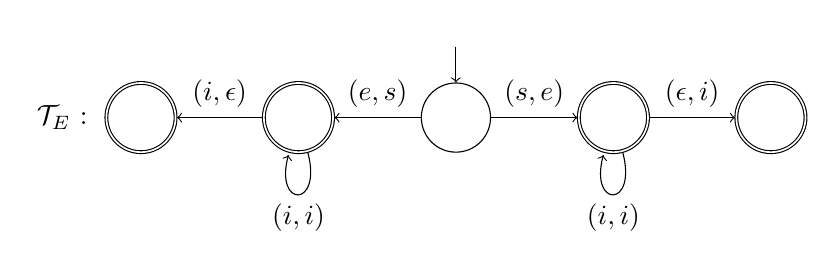
\begin{tikzpicture} [
						node distance=2cm, 
						auto,
						every initial by arrow/.style={->}
					]
					
\node (1) [state, initial above, initial text=] {};
\node (2) [state, accepting, right of=1] {};
\node (3) [state, accepting, left of=1] {};
\node (4) [state, accepting, right of=2] {};
\node (5) [state, accepting, left of=3] {};
\node (0) [left of=5, xshift=1cm] {$\mathcal{T}_E$ :};

\path[->]
	(1) edge node {$(s,e)$}   (2)
	(1) edge node[anchor=south] {$(e,s)$}   (3)
	(2) edge [loop below] node {$(i,i)$} ()
	(3) edge [loop below] node {$(i,i)$} ()
	(2) edge node {$(\epsilon,i)$} (4)
	(3) edge node[anchor=south] {$(i,\epsilon)$} (5);
\end{tikzpicture}\\
En construisant de tels automates pour les ensembles $V_e$, $I$ et $F$, on a réduit notre problème infini à un problème fini.
\end{frame}

\begin{frame}
\frametitle{Représentation rationnelle}
L'objectif est maintenant de construire un automate $\mathcal{A}_{W_s}$ acceptant le langage des mots représentant les sommets de l'ensemble gagnant du système.\\[3mm]

$\rightarrow$ Synthèse inductive guidée par le contre-exemple.
\end{frame}

\subsection{Apprentissage}
\begin{frame}
\frametitle{Apprentissage : ensemble gagnant}
Afin de construire l'automate $\mathcal{A}_{W_s}$, nous allons définir rigoureusement ce qu'est un ensemble gagnant.

\begin{block}{Ensemble gagnant}
Soit un jeu de sûreté défini par les ensembles $V_s$, $V_e$, $I$ et $F$, l'\emph{ensemble gagnant} pour le système est l'ensemble $W_s$ tel que :
\begin{itemize}
\item (1) $I\subseteq W_s$ 
\item (2) $W_s\subseteq F$
\item (3) $\forall v\in W\cap V_s,$ $Succ(v)\cap W\neq\emptyset$ 
\item (4) $\forall v\in W\cap V_e,$ $Succ(v)\subseteq W$
\end{itemize}
Où \emph{Succ($v$)} est la fonction retournant les successeurs du sommet $v$.\\
\end{block}
Cet ensemble n'est pas garanti d'exister pour un jeu de sûreté.
\end{frame}

\begin{frame}
\frametitle{Apprentissage : SIGCE} % exemple vérif une condition
La \emph{synthèse inductive guidée par le contre-exemple} est une manière d'apprendre un automate sur base d'un échange entre un enseignant (qui connait le jeu) et un élève.\\[3mm]

Cet apprentissage se déroule à l'intérieur d'un boucle telle qu'à chaque étape,
\begin{itemize}
\item L'élève conjecture un automate voulant décrire l'ensemble gagnant et le soumet à l'enseignant.
\item L'enseignant vérifie la définition d'ensemble gagnant pour cet automate.
\begin{itemize}
\item Si un règle est enfreinte, il retourne un \emph{contre-exemple}.
\item Sinon, l'apprentissage s'arrête et l'automate correspond à l'ensemble gagnant.
\end{itemize}
\end{itemize}

\end{frame}

\begin{frame}
\frametitle{Apprentissage : enseignant} % exemple vérif une condition
Afin de vérifier les conditions de la définiton d'ensemble gagnant, l'enseignant utilise des opérations diverses sur les automates afin de construire de nouveaux automates et vérifie le langage de ceux-ci.\\[3mm]
Selon ces vérifications, l'enseignant retourne deux types de contre-exemples :
\begin{itemize}
\item Les contre-exemples \emph{positifs} (resp. \emph{négatifs}) : un mot $u$ tel que $u$ doit obligatoirement être accepté (resp. rejeté) par $\mathcal{A}_{W_s}$.
\item Les contre-exemples d'\emph{implication universelle} (resp. \emph{existentielle}) : une paire $(u, \mathcal{A})$ telle que si le mot $u$ est accepté par $\mathcal{A}_{W_s}$, alors tous les mots de $\mathcal{L}(\mathcal{A})$ (resp. au moins un) doivent aussi être acceptés.
\end{itemize}

\end{frame}

\begin{frame}
\frametitle{Apprentissage : élève} % SAT, formule boléenne
Afin de conjecturer un automate, l'élève va construire des problèmes de satisfiabilité de taille incrémentale, basés sur les contre-exemples reçus. La taille du problème va dépendre du nombre de sommets dans l'automate qu'il va essayer de conjecturer.\\[3mm]
Si un de ces problèmes est satisfiable, alors un \emph{modèle} pour ce problème permettra de construire un automate à soumettre à l'enseignant.
\end{frame}

\subsection{Représentation boléenne du problème}
\begin{frame}
\frametitle{Formules boléennes} % exemple d'une formule
Afin d'assurer la cohérence de l'automate avec les contre-exemples, l'élève va utiliser plusieurs variables bolèennes.
\begin{itemize}
\item $d_{p,a,q}$ : si cette variable est vraie, alors une transition du sommet $p$ vers le sommet $q$ par $a$ existera dans l'automate.
\item $f_q$ : si elle est vraie, le sommet $q$ sera un sommet acceptant.
\item $x_{u,q}$ : si elle est vraie, la lecture du mot $u$ par l'automate amènera sur l'état $q$.
\end{itemize}
Ainsi, la formule 
\begin{equation}
\label{boolPos}
\begin{aligned} \bigwedge_{u\in P} \bigwedge_{q\in Q} x_{u,q} \rightarrow f_q \end{aligned}
\end{equation} 
où $P$ contient les contre-exemples positifs, forcera les mots de ces contre-exemples à être accepté par l'automate.
\end{frame}

\subsection{Stratégie gagnante}
\begin{frame}
\frametitle{Traduction d'un modèle en un ensemble gagnant}
$\mathcal{A}_{W_s}=\{Q,\Sigma,q_0,\delta,F\}$ tel que :
\begin{itemize}
\item $Q=\{0,$ $...$ $n\}$ est fixé à l'avance, où $n$ est la valeur incrémentale du problème de satisfiabilité.
\item $\Sigma=\{s,e,i\}$ 
\item $q_0=0$
\item $\delta$ contient les transitions de $p$ vers $q$ par $a$ pour toute variable $d_{p,a,q}$ vraie dans le modèle.
\item $f_q$ contient chaque sommet $q$ tels que $f_q$ est vraie dans le modèle.
\end{itemize}
\end{frame}

\begin{frame}
\frametitle{Stratégie gagnante}
Si l'apprentissage s'arrête, alors l'ensemble gagnant retourné donne immédiatment une stratégie gagnante pour le système.\\[3mm]
Cependant, si un tel ensemble n'existe pas, alors l'apprentissage ne s'arrêtera jamais.\\[6mm]
$\rightarrow$ L'algorithme n'est que partiel (et, s'il s'arrête, est de l'ordre de \alert{$O(n2^{n^2})$} pour un ensemble gagnant décrit par un automate à $n$ sommets).
\end{frame}

\subsection{Exemple}
\begin{frame}
\frametitle{Exemple}
Premier automate conjecturé par l'élève, en l'absence de contre-exemple :
\begin{figure}[H]
\centering
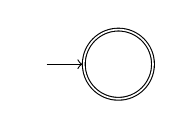
\begin{tikzpicture} [
						node distance=2cm, 
						auto,
						every initial by arrow/.style={->}
					]
								
\node (1) [state, initial, accepting, initial text=] {};
\end{tikzpicture}
\end{figure}
L'enseignant retourne un contre-exemple positif : $sii$.\\
Sur base de ce contre-exemple, l'élève soumet l'automate 
\begin{figure}[H]
\centering
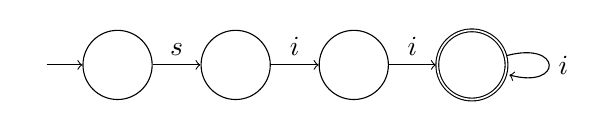
\begin{tikzpicture} [
						node distance=1.5cm, 
						auto,
						every initial by arrow/.style={->}
					]
								
\node (1) [state, initial, initial text=] {};
\node (2) [state, right of=1] {};
\node (3) [state, right of=2] {};
\node (4) [state, accepting, right of=3] {};

\path[->]
	(1) edge node {$s$}   (2)
	(2) edge node {$i$}   (3)
	(3) edge node {$i$}   (4)
	(4) edge [loop right] node {$i$} ();
	
\end{tikzpicture}
\end{figure}
à l'enseignant.
\end{frame}

\begin{frame}
\frametitle{Exemple}
L'enseignant retourne un contre-exemple d'implication existentielle $(sii, \mathcal{A})$ avec $\mathcal{L}(\mathcal{A})=\{eiii\}$.\\
L'élève retourne ensuite l'automate 
\begin{figure}[H]
\centering
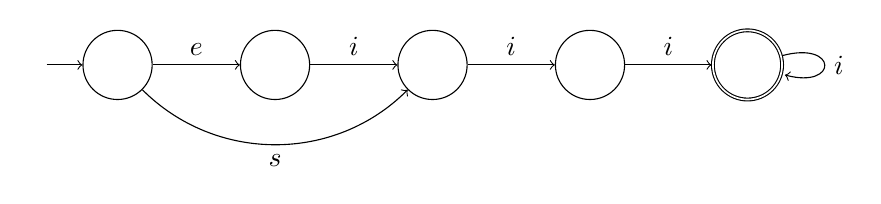
\begin{tikzpicture} [
						node distance=2cm, 
						auto,
						every initial by arrow/.style={->}
					]
								
\node (0) [state, initial, initial text=] {};
\node (1) [state, right of=0] {};
\node (2) [state, right of=1] {};
\node (3) [state, right of=2] {};
\node (4) [state, accepting, right of=3] {};

\path[->]
	(0) edge [out=315, in=225] node[anchor=north] {$s$}   (2)
	(0) edge node {$e$}   (1)
	(1) edge node {$i$}   (2)
	(2) edge node {$i$}   (3)
	(3) edge node {$i$}   (4)
	(4) edge [loop right] node {$i$} ();
	
\end{tikzpicture}
\end{figure}
L'enseignant ne trouve pas de contre-exemple à retourner car la définition d'ensemble gagnant est respéctée. L'apprentissage s'arrête.
\end{frame}

\section{Questions}
\begin{frame}
\frametitle{Questions}
Avez-vous des questions ?
\end{frame}

\section*{Remerciements}
\begin{frame}
\frametitle{Remerciements}
Merci à Gaëtan Staquet, Clément Tamines,\\
et plus particulièrement à Véronique Bruyère,\\
pour leur attention et leur suivi au cours de ce mémoire.
\vfill
\hfill Florent Huylenbroeck.
\end{frame}
\end{document}